\documentclass[conference]{IEEEtran}
\IEEEoverridecommandlockouts
\usepackage[utf8]{inputenc}
\usepackage{cite}
\usepackage{amsmath,amssymb,amsfonts}
\usepackage{graphicx}
\usepackage{booktabs}
\usepackage{url}

\begin{document}

\title{Optimizing Fire Station Expansion in Istanbul to Reduce Emergency Response Time}

\author{
\IEEEauthorblockN{Hikmet Gultekin}
\IEEEauthorblockA{AI and Data Engineering\\
Istanbul Technical University\\
gultekinh22@itu.edu.tr}
\and
\IEEEauthorblockN{Ata Turkoglu}
\IEEEauthorblockA{AI and Data Engineering\\
Istanbul Technical University\\
turkoglua21@itu.edu.tr}
\and
\IEEEauthorblockN{Azizagha Majidov}
\IEEEauthorblockA{AI and Data Engineering\\
Istanbul Technical University\\
majidov23@itu.edu.tr}
}

\maketitle

\begin{abstract}
This project studies where a limited number of additional fire stations should be opened in Istanbul. The model keeps existing stations active and selects new district-level candidate sites to reduce response time. To address the risk that average response-time minimization can leave distant districts underserved, we solve a weighted p-median benchmark and then an equity refinement that minimizes the worst district response within a bounded loss in average performance. All service costs are expressed in minutes through a single travel-time interface, preventing an inconsistency between road-time and Euclidean-distance objectives.
\end{abstract}

\section{Introduction}
Emergency response time is a public-safety measure in dense cities such as Istanbul. The project follows the submitted proposal and formulates fire station expansion as a location-allocation problem. The practical question is: given the current station network, which additional district-level sites most improve service, and how much equity is lost if only the total weighted response time is minimized?

\section{Problem Formulation}
Let $I$ be demand districts and $J$ be candidate service sites. Each district $i$ has weight $w_i$ from population. The service cost $t_{ij}$ is measured in minutes. Existing stations are fixed by $e_j=1$. The p-median model is
\begin{align}
\min & \sum_{i \in I}\sum_{j \in J} w_i t_{ij} y_{ij}\\
\textrm{s.t. } & \sum_{j \in J} y_{ij}=1 && \forall i \in I,\\
& y_{ij}\le x_j && \forall i,j,\\
& x_j \ge e_j && \forall j,\\
& \sum_{j \in J}(x_j-e_j)=p,\\
& x_j,y_{ij}\in\{0,1\}.
\end{align}
To avoid large gaps between districts, we add $r_i=\sum_j t_{ij}y_{ij}$ and solve a second-stage equity model:
\begin{align}
\min & \tau\\
\textrm{s.t. } & r_i \le \tau && \forall i,\\
& \sum_{i,j} w_i t_{ij}y_{ij} \le (1+\epsilon) Z^\star,
\end{align}
where $Z^\star$ is the p-median optimum and $\epsilon=0.02$ by default.

\section{Data and Preprocessing}
The pipeline downloads official Istanbul Metropolitan Municipality data: fire station locations, district population, average fire-event arrival time, first-degree emergency roads, and mukhtar office point locations. District demand points are centroids aggregated from 963 official neighborhood office points. Candidate sites are district centroids, while all existing stations remain active.

Full road routing is implemented as an optional OSMnx/NetworkX layer. When the road graph cannot be retrieved, the project uses a calibrated geometric proxy in minutes. The proxy is scaled so the baseline weighted average matches the IBB average arrival-time record. This same minute-scale model is used by the discrete, heuristic, and continuous optimization stages.

\section{Algorithmic Workflow}
The exact benchmark is solved with PuLP when available. In the submitted environment, PuLP is optional, so the notebook uses exact enumeration over district candidates; this is still exact for the 39-district candidate set and budgets $p\in\{1,3,5\}$. Genetic Algorithm and Simulated Annealing use fixed-size candidate subsets and an equity-aware score. Continuous refinement samples local points around a selected district site, fits a quadratic response-time surrogate in minutes, applies steepest descent and Newton updates with golden-section line search, then snaps the result to a feasible official neighborhood point.

\section{Experimental Evaluation}
\begin{table}[t]
\centering
\caption{Response-time comparison. Avg, P90, and Max are minutes. Coverage is weighted demand share within 8 minutes.}
\label{tab:results}
\IfFileExists{results_table.tex}{\begin{tabular}{lrrrrr}
\hline
Method & $p$ & Avg & P90 & Max & Cov. $\leq 8$ min\\
\hline
Current network baseline & 0 & 6.98 & 12.94 & 22.50 & 60.4\%\\
P-median & 1 & 6.56 & 12.08 & 22.50 & 63.7\%\\
Equity-refined p-median & 1 & 6.56 & 12.08 & 22.50 & 63.7\%\\
P-median & 3 & 5.86 & 12.08 & 22.50 & 71.4\%\\
Equity-refined p-median & 3 & 5.93 & 10.04 & 22.50 & 68.3\%\\
P-median & 5 & 5.23 & 9.93 & 22.50 & 76.0\%\\
Equity-refined p-median & 5 & 5.31 & 9.18 & 22.50 & 73.8\%\\
\hline
\end{tabular}
}{
\begin{tabular}{lrrrrr}
\hline
Method & $p$ & Avg & P90 & Max & Cov. $\leq 8$ min\\
\hline
Baseline & 0 & -- & -- & -- & --\\
\hline
\end{tabular}}
\end{table}

\begin{figure}[t]
\centering
\IfFileExists{figures/final_solution_map.png}{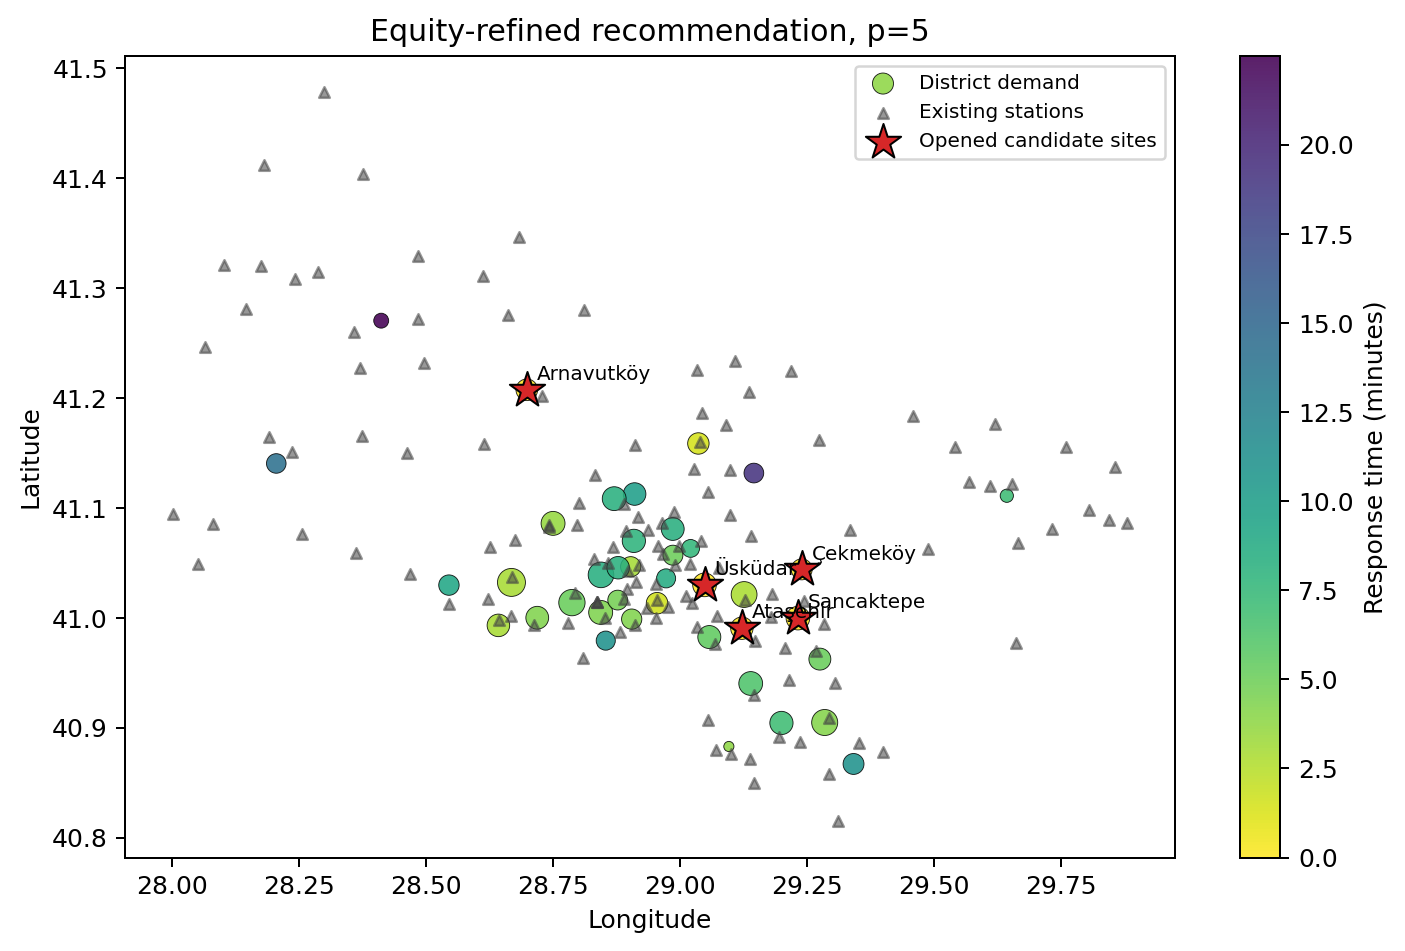
\includegraphics[width=\linewidth]{figures/final_solution_map.png}}{}
\caption{Equity-refined station expansion map. Larger district markers indicate higher population; color indicates response time in minutes.}
\label{fig:map}
\end{figure}

The p-median objective improves the population-weighted average response time. The equity refinement exposes the tradeoff between average performance and district-level gaps. If the 2 percent bound is too strict to improve the maximum response district, the sensitivity table in the notebook reports larger $\epsilon$ settings and the budget bisection experiment identifies how much additional budget is needed to meet a policy coverage target.

\begin{table}[t]
\centering
\caption{Equity tolerance sensitivity for $p=5$. A small increase in average-time tolerance can sharply reduce the worst district response.}
\label{tab:sensitivity}
\IfFileExists{sensitivity_table.tex}{\begin{tabular}{rrrr}
\hline
$\epsilon$ & Avg & P90 & Max\\
\hline
2\% & 5.31 & 9.18 & 22.50\\
5\% & 5.46 & 10.04 & 14.21\\
10\% & 5.61 & 10.04 & 12.94\\
\hline
\end{tabular}
}{}
\end{table}

\section{Real-World Application}
The model can support municipal planning by comparing expansion budgets, identifying underserved districts, and testing emergency-road disruption scenarios. The equity layer is important for public-safety use because low-population peripheral districts can be ignored by a pure average objective.

\section{Conclusion}
The project implements a proposal-faithful p-median fire station expansion pipeline and extends it with fairness diagnostics, heuristic comparisons, interactive controls, and continuous local refinement. The main methodological correction is consistency: every objective is evaluated in minutes, and Euclidean geometry is used only as a calibrated travel-time proxy when road routing is unavailable.

\begin{thebibliography}{00}
\bibitem{hakimi} S. L. Hakimi, ``Optimum locations of switching centers and the absolute centers and medians of a graph,'' \emph{Operations Research}, vol. 12, no. 3, pp. 450--459, 1964.
\bibitem{toregas} C. Toregas, R. Swain, C. ReVelle, and L. Bergman, ``The location of emergency service facilities,'' \emph{Operations Research}, vol. 19, no. 6, pp. 1363--1373, 1971.
\bibitem{church} R. Church and C. ReVelle, ``The maximal covering location problem,'' \emph{Papers in Regional Science}, vol. 32, no. 1, pp. 101--118, 1974.
\bibitem{bolouri} S. Bolouri, A. Vafaeinejad, A. A. Alesheikh, and H. Aghamohammadi, ``The ordered capacitated multi-objective location-allocation problem for fire stations using spatial optimization,'' \emph{ISPRS International Journal of Geo-Information}, vol. 7, no. 2, p. 44, 2018.
\bibitem{ibb} Istanbul Metropolitan Municipality, ``IBB Open Data Portal,'' 2026. [Online]. Available: \url{https://data.ibb.gov.tr/}
\end{thebibliography}

\end{document}
